%\documentclass[letterpaper, 10 pt, conference]{ieeeconf}`
%\usepackage{filecontents,lipsum}
%\usepackage[noadjust]{cite}
%%\begin{filecontents*}{references.bib}
%%@article{Khoe:1994:CML:2288694.2294265,
%%    author = {Khoe, G. -D.},
%%    title = {Coherent multicarrier lightwave technology for flexible capacity networks},
%%    journal = {Comm. Mag.},
%%    issue_date = {March 1994},
%%    volume = {32},
%%    number = {3},
%%    month = mar,
%%    year = {1994},
%%    issn = {0163-6804},
%%    pages = {22--33},
%%    numpages = {12},
%%    url = {http://dx.doi.org/10.1109/35.267438},
%%    doi = {10.1109/35.267438},
%%    acmid = {2294265},
%%    publisher = {IEEE Press},
%%    address = {Piscataway, NJ, USA},
%%}
%%\end{filecontents*}
%\title{This document}
%\author{This author}

%%%%%%%%%%%%%%%%%%%%%%%%%%%%%%%%%%%%%%%%%%%%%%%%%%%%%%%%%%%%%%%%%%%%%%%%%%%%%%%%
%2345678901234567890123456789012345678901234567890123456789012345678901234567890
%        1         2         3         4         5         6         7         8

\documentclass[letterpaper, 10 pt, conference]{ieeeconf}  % Comment this line out if you need a4paper

%\documentclass[a4paper, 10pt, conference]{ieeeconf}      % Use this line for a4 paper

\IEEEoverridecommandlockouts                              % This command is only needed if 
                                                          % you want to use the \thanks command

\overrideIEEEmargins                                      % Needed to meet printer requirements.

% See the \addtolength command later in the file to balance the column lengths
% on the last page of the document

% The following packages can be found on http:\\www.ctan.org
%\usepackage{graphics} % for pdf, bitmapped graphics files
%\usepackage{epsfig} % for postscript graphics files
%\usepackage{mathptmx} % assumes new font selection scheme installed
%\usepackage{times} % assumes new font selection scheme installed
%\usepackage{amsmath} % assumes amsmath package installed
%\usepackage{amssymb}  % assumes amsmath package installed
%\usepackage{filecontents,lipsum}
%\usepackage[noadjust]{cite}
%\usepackage{bm}
%\usepackage{tikz}
%\usepackage{graphicx}
%\usepackage{caption}
%\usepackage{subcaption}
%\usepackage{multicol}
%\usepackage{url}
%\usepackage{geometry}
%\usepackage{mathtools}
%\usepackage[utf8]{inputenc}
%\usepackage[english]{babel}
%\usepackage{algorithm}
%\usepackage[]{algpseudocode}


\usepackage{afterpage}
\usepackage{algorithm}
\usepackage[]{algpseudocode}

\usepackage{stix}
%\usepackage{amssymb} %redundant with stix
\usepackage{amsmath}

% \DeclareMathAlphabet\mathcal{OMS}{cmsy}{b}{n}
%\usepackage[math-style=TeX, bold-style=TeX]{unicode-math}
% \DeclareMathAlphabet{\pazocal}{OMS}{zplm}{m}{n}
% \newcommand{\unif}{\pazocal{U}}

\DeclareSymbolFont{cmsymbols}{OMS}{cmsy}{m}{n}
\SetSymbolFont{cmsymbols}{bold}{OMS}{cmsy}{b}{n}
\DeclareSymbolFontAlphabet{\mathcal}{cmsymbols}

\usepackage{arydshln}
\usepackage[english]{babel}
\usepackage{bm}
\usepackage{caption}
\usepackage[T1]{fontenc}
\usepackage[]{graphicx}
\graphicspath{ {./fig/} }

\usepackage[utf8]{inputenc}
\usepackage{marginnote}
\usepackage{multicol}
\usepackage{xcolor}
%\usepackage[T1]{xcolor} %T1 is not used with xcolor
\usepackage{soul}
\usepackage{subfig}
\usepackage{tikz}
\usepackage{url}
\usepackage[backend=biber,style=ieee,sorting=none]{biblatex}
\addbibresource{bib/references.bib}


\newcommand{\trsp}{{^{\top}}}

\newcommand\blankpage{%
    \null
    \thispagestyle{empty}%
    \addtocounter{page}{-1}%
    \newpage}

\newcommand*\circled[1]{\tikz[baseline=(char.base)]{
            \node[shape=circle,draw,inner sep=2pt] (char) {#1};}}

\newcommand*{\important}[1]{\textcolor{red}{\danger~\textbf{IMPORTANT:~}} \textcolor{red}{#1}}

\newcommand*{\pending}[1]{\textcolor{blue}{$\bigstar$~\textbf{PENDING~#1}}}

\newcommand\mybox[2][]{\tikz[overlay]\node[fill=blue!100,inner sep=4pt, anchor=text, rectangle, rounded corners=1mm,#1] {#2};\phantom{#2}}

\newcommand{\TODO}{\mybox[fill=yellow]{\textcolor{blue}{\Large \textbf{TODO}}}}
\newcommand\myhl[1]{\textcolor{red}{#1}}


\newtheorem{prop}{Proposition}

\usepackage[nolist]{acronym}
\newacro{smc}[SMC]{sensorimotor contingencies}
\newacro{dfc}[DFC]{dynamic functional connectivity}
\newacro{fc}[FC]{functional connectivity}
\newacro{nnmf}[NNMF]{non-negative matrix factorization}
\newacro{imi}[IMI]{instantaneous mutual information}
\newacro{irm}[IRM]{infinite relational model}
\newacro{mi}[MI]{mutual information}

\newacro{}[]{}
\newacro{}[]{}
\newacro{}[]{}

\title{\LARGE \bf
An analytical framework for the discovery of body features and behaviors from sensorimotor dynamic functional connectivity
}


\author{Fernando D\'iaz Ledezma$^{1,\dagger}$, Valentin Marcel$^{2,\dagger}$, and Matej Hoffmann$^{2}$% <-this % stops a space
\thanks{V.M. and M.H. were supported by Czech Science Foundation (GA CR), projects 20-24186X and 25-18113S.  F.D.L. acknowledges the funding by the Deutsche Forschungsgemeinschaft through the Gottfried Wilhelm Leibniz Programme (awarded to Sami Haddadin; grant no. HA7372/3-1). The work initiated during the stay of F.D.L. at CTU, supported by the OP VVV MEYS funded project CZ.02.1.01/0.0/0.0/16\_019/0000765.}% <-this % stops a space
\thanks{$^{1}$Fernando D\'iaz Ledezma is with the School of Computation, Information and Technology, Technical University of Munich, Munich, Germany {\tt\small fernando.diaz@tum.de}}%
\thanks{$^{2}$Valentin Marcel and Matej Hoffmann are with the Faculty of Electrical Engineering, Czech Technical University in Prague, Prague, Czech Republic
        {\tt\small \{valentin.marcel,matej.hoffmann\}@fel.cvut.cz}}%
\thanks{$^\dagger$ The authors contributed equally to this work.}
}


\begin{document}
\maketitle
% ---
\begin{figure*}[h!]
	\centering
	\includegraphics[width=0.95\textwidth]{sensorimotor_dfc_framework.png}
	\caption{\textbf{From the sensorimotor \acl{dfc} to motor behaviors.} Random motion (babbling) excites the sensorimotor system of the robotic agent. While moving, the \ac{imi} captures the changing sensorimotor \ac{fc} over time. The \ac{irm} captures clusters of signals from the \ac{imi} and their corresponding dynamic relationships. Finally, \ac{nnmf} decomposes these relationships into basis factors signifying underlying motor behavior patterns present in the original data.}
	\label{fig:framework_overview}
\end{figure*}
% ---
\begin{abstract}
Movements of both animals and robots give rise to streams of high-dimensional motor and sensory information. Imagine the brain of a newborn or the controller of a baby humanoid robot trying to make sense of unprocessed sensorimotor time series. Here we present a framework for studying the dynamic functional connectivity among an embodied agent’s multimodal sensory signals to uncover an underlying structure. By leveraging instantaneous mutual information, we captured the time-varying functional connections between proprioceptive, tactile, and visual signals, revealing the sensorimotor relationships. Through the application of an infinite relational model, we identified sensorimotor modules and their evolving connectivity. To further interpret these dynamic interactions, we employed non-negative matrix factorization, which decomposed the connectivity patterns into additive factors and their corresponding temporal coefficients. These factors can be considered the agent’s motion primitives or movement synergies that the agent can use to make sense of its sensorimotor space and later for behavior selection. In the future, the method can be deployed in robot learning as well as in the analysis of human movement trajectories or brain signals.


%Regularities present in the somatosensory signals of a robotic agent can reflect its embodiment and the associations resulting from an active control policy. In this work, we analyze the dynamic functional connectivity of the somatosensory signals based on the instantaneous pairwise mutual information. As the robot performs exploratory motions based on motor babbling, we capture and study the time-varying changes in the signal relationships. We analyze the instantaneous and average information sharing and associate them with different information states. A simulated planar system study shows that using instantaneous mutual information to extract and leverage the relationships between the agent's somatosensory signals exhibited during exploratory motions can yield information related to self-touch events.
\end{abstract}
% =============================================================================
%                                                                             |
%                                                                             |
% ------------------------------- SECTION ------------------------------------|
%                                                                             |
%                                                                             |
% =============================================================================
\section{Introduction}\label{sec:intro}
Understanding the brain’s structural and \ac{fc} has significantly advanced our knowledge of its organization and information-processing capabilities. A similar approach can be applied to studying the sensorimotor signals of an embodied agent, offering insights into how the agent processes information and adapts its behavior. While analyzing the structural connectivity of these signals may not always be feasible, investigating their functional connectivity provides a powerful way to understand an agent’s body structure and the emergence of behavior through information acquisition. A key concept in this context is that of \ac{smc} \cite{oregan2001sensorimotor}, the regularities and dependencies between an organism's actions (motor actions) and the resulting sensory feedback linking an agent’s sensorimotor signals to its physical embodiment and the world. Identifying and analyzing these regularities using information-theoretic methods can help uncover fundamental principles of sensorimotor learning. 


% SUBSECTION ==================================================================
\subsection{Related works}
Research suggests that \acp{smc} play a fundamental role in acquiring body knowledge, generalization, and goal-directed behavior \cite{Jacquey2019Sensorimotorcontingenciesas}. As such, they can be viewed as a form of sensorimotor representation---a framework that enables an embodied agent to learn, adapt, and interact with its environment. Despite extensive research on sensorimotor representations \cite{Nguyen2021Sensorimotorrepresentationlearning}, the precise relationship between sensorimotor regularities, body knowledge, and behavior remains an open question.

% Several studies have used information-theoretic metrics to examine these relationships in sensorimotor systems \cite{Schmidt2013Bootstrappingperceptionusing,Lungarella2006Mappinginformationflow,Polani2009Modelsinformationprocessing,Olsson2006unknownsensorsactuators}. 
Several studies have used information-theoretic metrics to examine these relationships in sensorimotor systems. 
For example, \ac{mi} was used by D\'iaz et al. \cite{DiazLedezma2023MachineLS} to discover the mechanical topology of a robot from its proprioceptive signals. Touch has been identified as crucial in understanding \acp{smc} among different sensory modalities. Gama et al. \cite{Gama2021Goaldirectedtactile} demonstrated how intrinsic motivation and goal-babbling can facilitate self-touch learning in a simulated humanoid robot with artificial tactile skin. Similarly, Roncone et al. \cite{Roncone2014Automatickinematicchain} showed that self-touch could be used for kinematic calibration, allowing a robot to close its kinematic chain autonomously by touching its own body. Marcel et al. \cite{Marcel2022Learningreachown} further explored self-touch representation using a denoising framework with a multimodal variational autoencoder, enabling a robot to reconstruct its self-reaching configurations internally.

Another relevant area of study is \ac{dfc}, which explores how the statistical properties of sensorimotor signals evolve over time. Originally applied in neuroscience, \ac{dfc} has been used to detect states of reduced functional connectivity during epilepsy onsets \cite{Christiaen2020Dynamicfunctionalconnectivity} and to identify abnormal connectivity patterns in brains affected by illness \cite{Zhou2020Earlychildhooddevelopmental}. More recently, \ac{dfc} has been used to investigate how sensorimotor connectivity evolves in infants as they develop \cite{Kanazawa2023Openendedmovements}.

In robotics, functional connectivity is expected to change based on the robot’s motion policy or the task it performs. Capturing and analyzing these evolving patterns using \ac{dfc} could provide a deeper understanding of how an agent’s sensory and motor systems interact over time.

% SUBSECTION ==================================================================
\subsection{Overview}
This work introduces an analytical framework, illustrated in Fig.~\ref{fig:framework_overview}, to investigate the formation of relationships between the sensorimotor signals of a simulated two-dimensional embodied agent. Specifically, the framework examines the time-varying \acl{fc} between the agent's proprioceptive, tactile, and visual inputs. During an initial exploratory phase using motor babbling, the agent gathers information about its evolving sensorimotor relationships. The framework models these changing relationships as time-varying graphs, serving as a proxy for understanding the formation and evolution of \acp{smc}. To achieve this, we compute the instantaneous pairwise \ac{mi} between sensorimotor signals, capturing the \acl{dfc} that correlates the agent’s information-sharing state with its motion and potential interactions. A key step in the framework involves applying a Bayesian approach to uncover hidden structures within the mutual information-based connectivity. This analysis identifies clusters of highly related signals and their evolving interactions over time. Finally, the framework decomposes these dynamic relationships to extract meaningful patterns (i.e., subgraphs) in the graphs, which represent distinct information-sharing states. The insights derived from these states and their transitions reveal fundamental aspects of the agent’s body structure and behavior.
% ---
\begin{figure}[!t]
	\begin{center}
		\hspace*{\fill}
		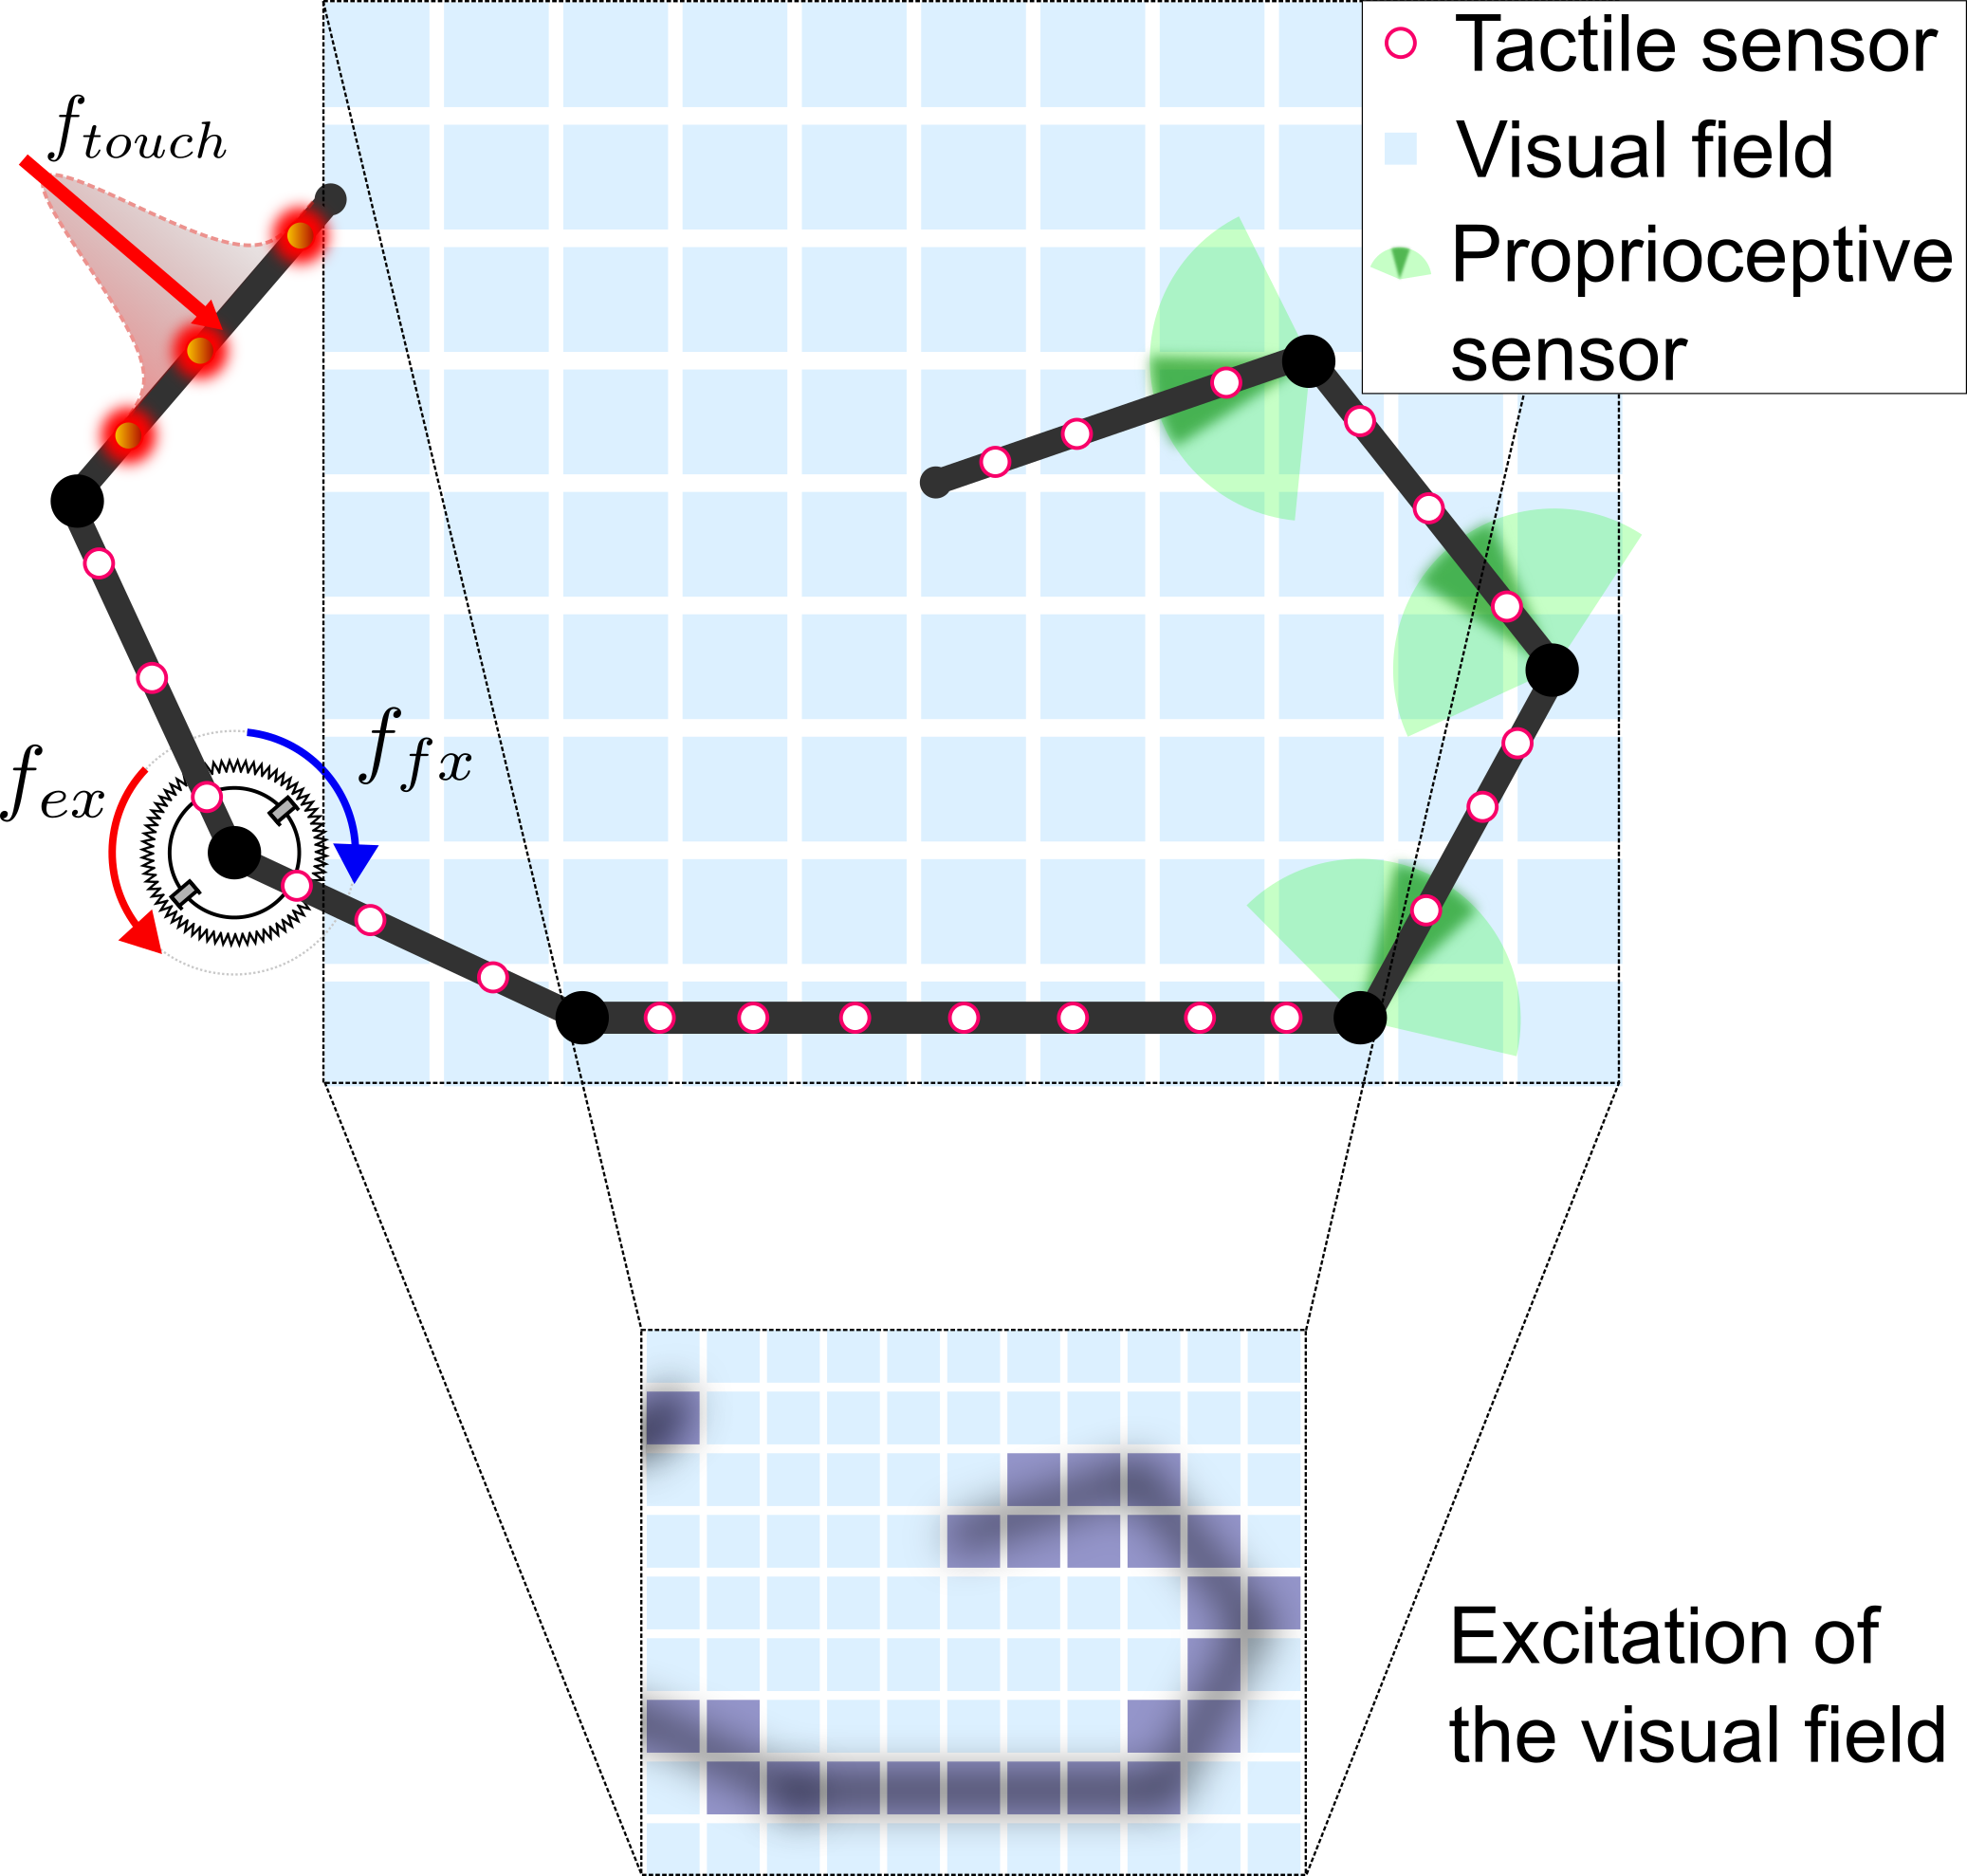
\includegraphics[width=0.99\columnwidth]{extended_planar_dual_arm_with_vision_v2.png}
		\hspace*{\fill}
	\end{center}
	\caption{\label{fig:extended_dual_arm_robot} \textbf{The embodied agent.} The planar dual arm robot is driven by antagonistic actuation in each joint. Sensory information comes from tactile and proprioceptive receptive fields along the body and at the joints. The visual field (gray area) detects parts of the body when inside it.}
\end{figure}
% ---

% =============================================================================
%                                                                             |
%                                                                             |
% ------------------------------- SECTION ------------------------------------|
%                                                                             |
%                                                                             |
% =============================================================================
\section{The embodied agent}\label{sec:the_embodied_agent}
% SUBSECTION ==================================================================
\subsection{The planar dual arm model}
We started from the model described in \cite{Mannella2018Knowyourbody} and used also in \cite{Marcel2022Learningreachown}, adding population code of the sensory receptors. This model consists of a simple planar dual-arm system with six degrees of freedom, featuring three links per arm and a fixed torso, see Fig.~\ref{fig:extended_dual_arm_robot}. The robot is equipped with tactile sensors distributed across its body. 

In this work, we extended the model as follows. 
To instantiate the dynamics of the model, inertial properties are assigned to the robot's composing bodies. Its actuation mechanism is based on a biologically-inspired model presented in \cite{Shim2012Chaoticexplorationlearning}, where the position $q$ and velocity $\dot{q}$ of each joint is driven by antagonistic muscles (modeled as spring-damper systems). The pulling force these muscles exert is linearly controlled by the signal generated by a corresponding motor neuron $\sigma$. The joint torque,
% ---
\begin{equation}\label{eq:antagonistic_torque}
	\tau = \alpha \left(\sigma_\mathrm{fx} - \sigma_\mathrm{ex}\right)  + \beta \left(\sigma_\mathrm{fx} + \sigma_\mathrm{ex} + \gamma \right) q + \delta \dot{q},
\end{equation}
% ---
results from the difference between activation signals for flexion $ \sigma_\mathrm{fx} $ and extension $\sigma_\mathrm{ex}$. These activation signals contribute to the flexion and extension pulling forces, $ f_\mathrm{fx}$ and $f_\mathrm{ex} $, respectively. The remaining parameters in the model account for the muscle force gain ($\alpha$), stiffness gain ($\beta$), tonic stiffness ($\gamma$), and damping coefficient ($\delta$).

% SUBSECTION ==================================================================
\subsection{The sensory signals}
%Randomly located tactile sensors along the robot's one-dimensional body are modeled based on population coding \cite{Panzeri2010PopulationCoding}. They are represented as distance-dependent Gaussian receptive fields---see Fig.~\ref{fig:population_coding}---whose mean is dictated by the tactile sensor location. 
%To incorporate touch strength into the model, we adjust the distance-based activation of the Gaussian receptive fields based on the contact force. Similarly, the proprioceptive measurements of the robot are also encoded using receptive fields. Ultimately, our extended model results in a vector $\bm{s}$ containing a number $N_s$ of somatosensory signals encompassing proprioception (joint position $\bm{p}$, velocity $\bm{v}$, and effort $\bm{e}$) and touch-strength-modulated tactile signals $\bm{r}$; i.e.:
%% ---
%\begin{equation}
%	\bm{s} = \begin{bmatrix}
%		\bm{p}\trsp & \bm{v}\trsp & \bm{e}\trsp & \bm{r}\trsp
%	\end{bmatrix}\trsp \in \mathbb{R}^{N_s}_{\geq}.
%\end{equation}
%%---
%\myhl{In addition to somatosensation, we equip the robot with visual inputs. The visual sensors are composed of a fixed, rectangular, pixel grid of size $(s_\text{x},s_\text{y})$ with  $(n_\text{x},n_\text{y})$ pixels in each direction. Pixels are sensitive to the positions of the agent's limbs; e.g., when a limb segment intersects with the rectangular pixel receptive field in the 2D space, its value is updated to one. To simulate some visual sensors' spatial overlap~\cite{Marshall2015}, we perform a convolution of the pixel values image with a 3-by-3 kernel mapping to get the visual sensors' activations.}

%Randomly located tactile sensors along the robot's one-dimensional body are modeled based on population coding \cite{Panzeri2010PopulationCoding}. They are represented as distance-dependent Gaussian receptive fields---see Fig.~\ref{fig:population_coding}---whose mean is dictated by the tactile sensor location. To incorporate touch strength into the model, we adjust the distance-based activation of the Gaussian receptive fields based on the contact force. Similarly, the proprioceptive measurements of the robot are also encoded using receptive fields. In addition to somatosensation, we equip the robot with visual inputs. The visual sensors are composed of a fixed pixel receptive field with $(n_\text{x},n_\text{y})$ pixels in each direction. When a limb segment intersects with a pixel in the visual field, its value is updated to one; i.e., the pixels are sensitive to the positions of the agent's limbs. Additionally, to simulate spatial overlap in some of the visual sensors~\cite{Marshall2015}, we perform a convolution of the pixel values image with a 3-by-3 kernel mapping to get the pixel receptive field's activations.
%
%Ultimately, in our extended model, $N_s$ signals encompassing position-based proprioception, touch-strength-modulated tactile sensation $\bm{r}$, and visual inputs $\bm{v}$ form a vector
%% ---
%\begin{equation}
%	\bm{s} = \begin{bmatrix}
%		\bm{p}\trsp & \bm{r}\trsp & \bm{v}\trsp
%	\end{bmatrix}\trsp \in \mathbb{R}^{N_s}_{\geq}.
%\end{equation}
%%---
%of somatosensory signals. In stage \circled{1} of our proposed analytical framework, perceptual system of the embodied agent is excited to collect the signals $\bm{s}$ following a motor babbling strategy. 


Tactile sensors are randomly distributed along the robot's one-dimensional body and modeled using population coding \cite{Panzeri2010PopulationCoding}. Each sensor is represented by a Gaussian receptive field, whose mean is determined by the sensor's location. %n—see Fig.~\ref{fig:population_coding}. 
To incorporate touch strength, we modulate the activation of each receptive field based on the contact force, adjusting the distance-dependent response accordingly.  

Similarly, the robot's proprioceptive measurements are also encoded using Gaussian receptive fields. In addition to somatosensation, the robot is equipped with visual inputs. The visual sensors consist of a fixed pixel receptive field with dimensions $(n_\text{x}, n_\text{y})$. When a limb segment intersects with a pixel in the visual field, the pixel value is set to one---i.e., pixels are sensitive to the positions of the agent's limbs. To account for the spatial overlap in some visual sensors~\cite{Marshall2015}, we apply a convolution operation using the 3-by-3 kernel \[
\small
K = \begin{bmatrix} 
0 & 0.25 & 0 \\ 
0.25 & 1 & .25 \\ 
0 & 0.25 & 0 
\end{bmatrix}
\] to the whole image followed by a saturation $\bm{v}=\texttt{min}(\bm{v},1)$ to keep the neural activations between $[0,1]$.

Ultimately, in our extended model, the visuo-somatosensory signal vector consists of $N_\text{s}$ signals, including position-based proprioception ($\bm{p}$), touch-strength-modulated tactile sensation ($\bm{r}$), and visual inputs ($\bm{v}$):  
% ---
\begin{equation}
	\bm{s} = \begin{bmatrix}
		\bm{p}\trsp & \bm{r}\trsp & \bm{v}\trsp
	\end{bmatrix}\trsp \in \mathbb{R}^{N_\text{s}}_{\geq}.
\end{equation}
%---
In stage \circled{1} of our proposed analytical framework, the perceptual system of the embodied agent is stimulated to collect the signals $\bm{s}$ through a motor babbling strategy.

%% ---
%\begin{figure}[!t]
%	\begin{center}
%		\hspace*{\fill}
%		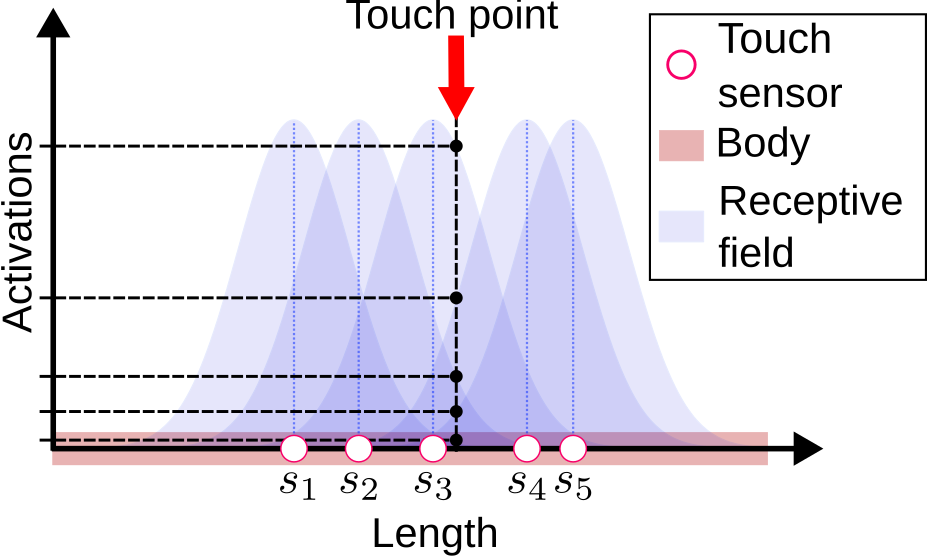
\includegraphics[width=0.75\columnwidth]{touch_receptive_fields.png}
%		\hspace*{\fill}
%	\end{center}
%	\caption{\label{fig:population_coding} \textbf{Population coding.} The receptive fields encode a signal into several distance-based activation functions.}
%\end{figure}
%% ---
% =============================================================================
%                                                                             |
%                                                                             |
% ------------------------------- SECTION ------------------------------------|
%                                                                             |
%                                                                             |
% =============================================================================
\section{The sensorimotor dynamic functional connectivity}

% Subsection ==================================================================
\subsection{\Acl{fc}}
\ac{fc} is a method for inferring network topology by characterizing the dependencies between observed signals based on their probability distributions \cite{Friston2011Functionaleffectiveconnectivity}. Analyzing \ac{fc} helps uncover underlying structures describing interactions between network entities. Building on the connection between embodiment and information structure \cite{Pfeifer2007Selforganizationembodiment}, we hypothesize that an embodied agent’s bodily structural properties and motor behaviors can be revealed by studying the \ac{fc} among its sensorimotor signals $\bm{s}(t)$. To quantify these relationships, we leverage information-theoretic measures, as their model-free nature captures both linear and nonlinear dependencies between signals. In particular, we focus on \ac{mi}, a widely used measure for quantifying relationships between variables across different domains \cite{Steuer2002mutualinformationdetecting}.

% Given the Shannon's entropy of a variable $X$  
% % ---
% \begin{equation}\label{eq:entropy}
% 	H(X) = -\sum_{i=1}^{n}p(x_i)\text{log}_2\left(p\left(x_i\right)\right)
% \end{equation}
% % ---
% and the joint entropy between two variables $ X $ and $ Y $ 
% % ---
% \begin{equation}\label{eq:joint_entropy}
% 	H(X,Y) = -\sum_{i=1}^{n}\sum_{j=1}^{n} p(x_i,y_j)\text{log}_2\big(p\left(x_i,y_j\right)\big),
% \end{equation}
% % ---
% the \ac{mi} between two signals 
% % ---
% \begin{equation}\label{eq:mutual_information}
% 	I\left(X;Y\right) =I\left(Y;X\right) = H(X) + H(Y) - H(X,Y)
% \end{equation}
% % ---
% can be interpreted as the amount by which a random signal $ Y $ reduces the uncertainty about a random signal $ X $ \cite{Cover1999Elementsinformationtheory}. It is a symmetric measure of the information sharing by both signals, depending on their marginal $p(\cdot)$ and joint $p(\cdot,\cdot)$ probability distributions.

The \ac{mi} between two signals $I\left(X;Y\right)$ can be interpreted as the amount by which a random signal $ Y $ reduces the uncertainty about a random signal $ X $ \cite{Cover1999Elementsinformationtheory}. It is a symmetric measure of the information sharing by both signals. By extension, the \ac{mi} matrix $\bm{\mathcal{I}} \in \mathbb{R}^{{N_\text{s}} \times {N_\text{s}}}$ can be constructed by computing the pairwise \ac{mi} between the $\left\lbrace s_i\right\rbrace^{N_\text{s}}_{i=1}$ sensorimotor signals. In practice, computing an entry
% ---
\begin{equation}\label{eq:adjacency_mi}
	\left(\bm{\mathcal{I}}\right)_{i,j} = I(s_i;s_j)
\end{equation}
% ---
for a pair $\left({s}_i(t),{s}_j(t)\right)$ involves centering their samples---to zero mean and unit standard deviation---and using either binning, kernel, or nearest neighbor methods to compute their \ac{mi} \cite{WaltersWilliams2009Estimationmutualinformation}.

% ---
\begin{figure}[!t]
	\begin{center}
		\hspace*{\fill}
		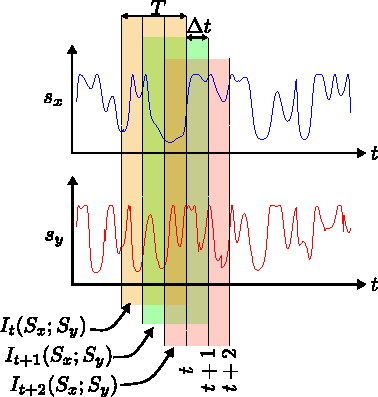
\includegraphics[width=0.7\columnwidth]{sliding_window_mi.pdf}
		\hspace*{\fill}
	\end{center}
	\caption{\label{fig:mi_sliding_window_mi} \textbf{\Acl{imi}.} A sliding window strategy is used to compute the \ac{mi} in an interval $\left[t-T,t\right]$.}
\end{figure}
% ---
% Subsection ==================================================================
\subsection{\Acl{dfc}}
When analyzing \ac{fc}, it might be interesting to look not only at the aggregated effect of a complete dataset of recordings but also at the instantaneous changes that occur in the relationships. Indeed, the functional relationships between sensorimotor signals can change rapidly depending on the motion policy and the agent's interaction with the environment. To capture this time-varying, i.e., dynamic, \acl{fc}, it is common to use a sliding time window \cite{Preti2017dynamicfunctionalconnectome} with forward step $\Delta t$ from which the \ac{mi} is computed only for a small number of samples.

For a time window of length $T$, the \ac{mi} $I_t(s_x(t);s_y(t))$ between a distinct pair of signals $s_x(t)$ and $s_y(t)$ at time $t$ is computed using the set of signal samples spanning the $\left[t-T,t\right]$ interval, as illustrated in Fig.~\ref{fig:mi_sliding_window_mi}. We refer to this quantity as the \acf{imi}. 

By extension, in stage $\circled{2}$ in Fig.~\ref{fig:framework_overview}, the \ac{mi} matrix $\bm{\mathcal{I}}(t)$ at time $t$ is constructed by calculating the \ac{imi} for all pairwise signals within the same time interval. The temporal evolution of this time-varying \ac{mi} matrix $\bm{\mathcal{I}}(t)$ captures the \ac{dfc} between the sensorimotor signals.

% Subsection ==================================================================
\subsection{Finding structure in the functional relationships}\label{sec:the_irm}
Analyzing the time-varying relationships in $\bm{\mathcal{I}}(t)$ at a local level may not be as informative as examining the global structure defined by interactions between groups of signals. To address this, we first identify clusters of closely related signals based on their \ac{mi} values. However, conventional clustering techniques typically require a predetermined number of clusters. To overcome this limitation, in stage \circled{3} of our framework, we employ a Bayesian approach---the \ac{irm}~\cite{Moerup2012}---to uncover hidden structures within the \ac{mi}-based connectivity.

This probabilistic framework groups entities (e.g., signals) into $N_\text{c}$ clusters while simultaneously learning the relationships between them. Its primary objective is to group entities into clusters based on their relationships and predict new relationships based on these assignments. The \ac{irm} utilizes a Chinese Restaurant Process or a Dirichlet Process, allowing the number of clusters to dynamically expand as needed. By leveraging probabilistic methods, the \ac{irm} estimates the likelihood of entities belonging to the same cluster and models inter-cluster relationships using probability distributions.

For our purposes, the \ac{irm} takes as an input the time series of  \ac{imi}-matrices---representing $N$ samples $\left\lbrace \bm{\mathcal{I}}(k)\right\rbrace^{N}_{k=1}$---and assigns to the i-th signal in $\bm{s}$ a cluster $z_i$. To identify these latent cluster relationships, \ac{irm} assumes that the probability of a relation between two entities depends only on their cluster memberships. Specifically, if two entities belong to clusters $z_i$ and $z_j$, the connection probability is determined by a parameter $\theta_{z_i,z_j}$. These inter-cluster probabilities form a new binary relational matrix $\bm{Z}\in \mathbb{R}^{N_\text{c}\times N_\text{s}}$, which the model infers from data. Additionally, the \ac{irm} produces a matrix array $\bm{H}\in \mathbb{R}^{N_\text{c}\times N_\text{c} \times N}_{\geq}$, which captures the probability of relations between clusters.

% Subsection ==================================================================
\subsection{Analyzing recurring patterns}
The matrices $(\bm{Z}, \bm{H})$ in Sec.~\ref{sec:the_irm} capture the global changing relationships between the sensorimotor signals. In stage $\circled{4}$, the goal is to utilize the $N$ relationships captured in $\bm{H}$ to identify recurrent patterns in the \ac{fc} that correspond to distinct motor behaviors of the agent. Additionally, assessing the strength and frequency of these patterns is crucial to determine their significance. 

Common approaches to detect repeating patterns in \ac{dfc} include the cosine similarity~\cite{Menon2019comparisonstaticdynamic}, k-means clustering~\cite{Li2017Hightransitionfrequencies}, and  \ac{nnmf}~\cite{Fu2019Nonnegativematrixfactorization}. We selected the latter due to its demonstrated effectiveness in analyzing brain dynamic functional networks and its application in community  detection~\cite{Luo2021Symmetricnonnegativematrix}.

To use \ac{nnmf}, a matrix $\bar{\bm{H}} = [\bar{\bm{h}}(1) \cdots \bar{\bm{h}}(k) \cdots \bar{\bm{h}}(N)] \in \mathbb{R}^{N_\text{r}\times N}$ is constructed by vectorizing and concatenating each of the matrices in $\bm{H}$ (i.e., a flattened version of the upper triangular part of $\bm{H}$); where $N_\text{r} = N_\text{c}(N_\text{c}-1)/2$. Since this matrix is strictly non-negative, it is amenable to be decomposed and analyzed using \ac{nnmf}. Then, the \ac{nnmf} algorithm can be used to factor the nonnegative matrix $\bar{\bm{H}}$ into two parts: a matrix $\bm{F} \in \mathbb{R}^{N_\text{f}\times N_\text{r}}_{\geq}$ of $N_\text{f}$ basis (or factors) and a matrix $\bm{W} \in \mathbb{R}^{N\times N_\text{f}}_{\geq}$ of their corresponding contributions, or scores, such that
% ---
\begin{equation}
	\bar{\bm{H}}^\intercal \approx \bm{W} \bm{F}.
    \label{eq:nnmf}
\end{equation}
% ---
%\begin{figure}[!t]
%	\centering
%	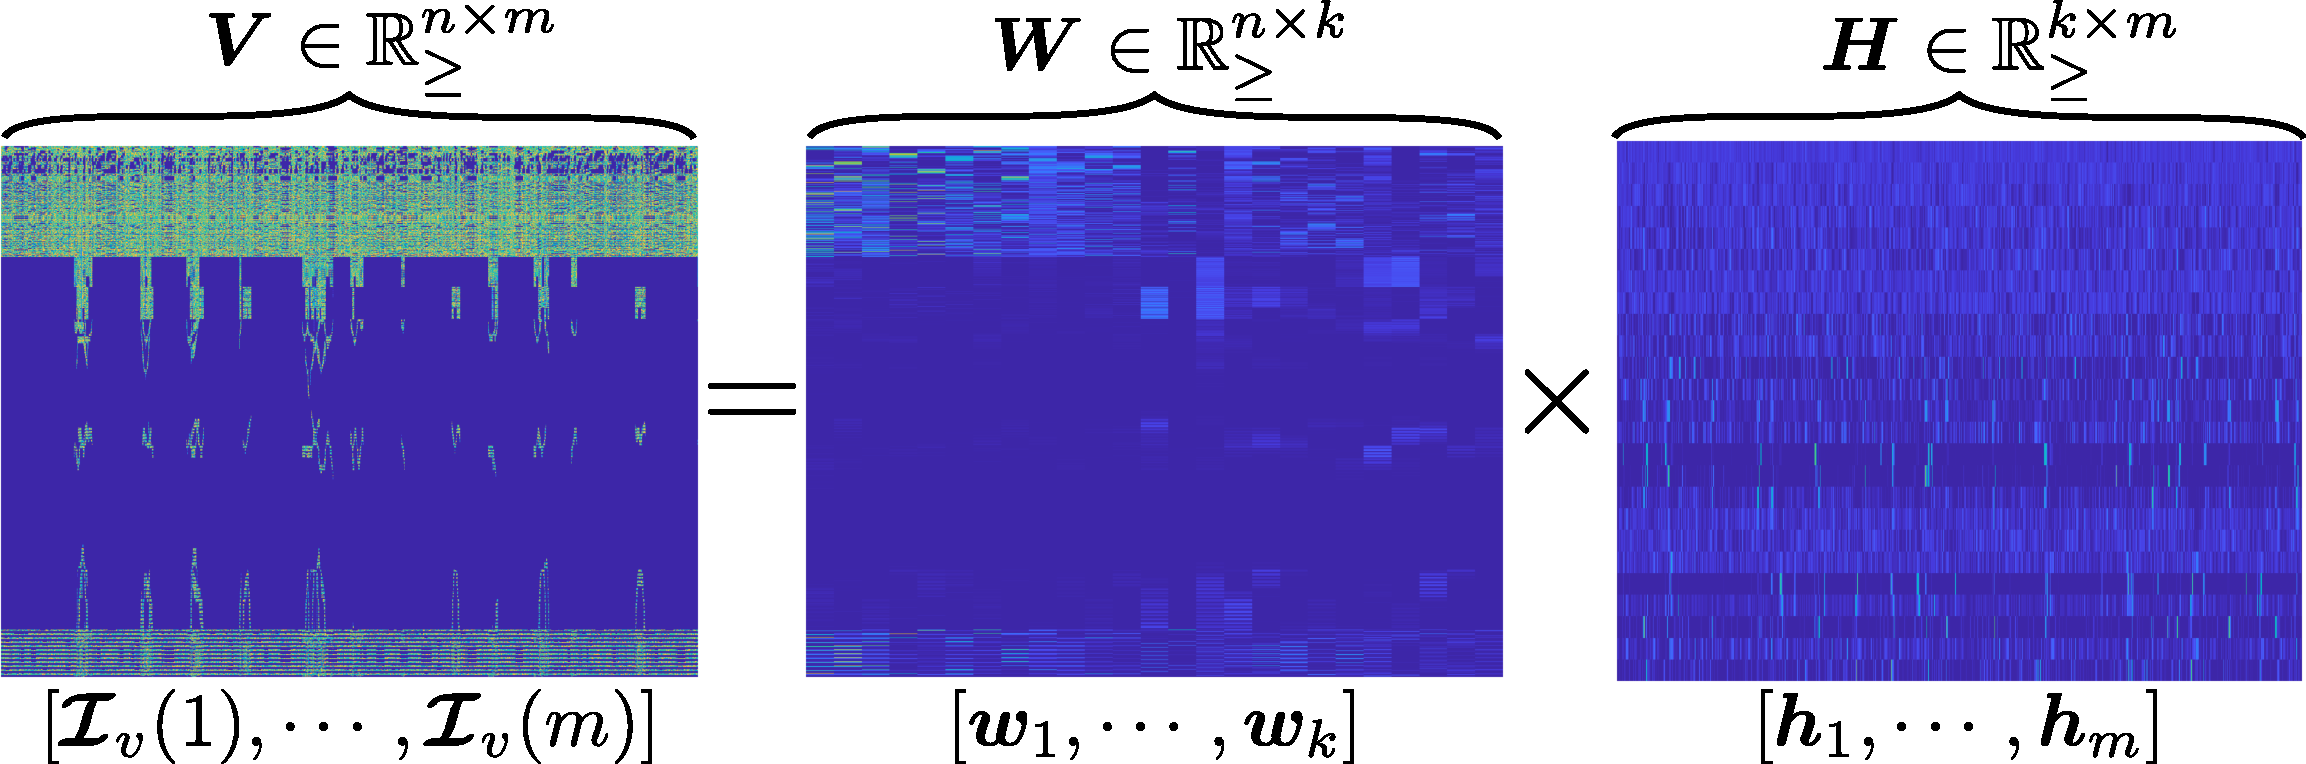
\includegraphics[width=0.99\columnwidth]{fig/nnmf_concept.pdf}
%	\caption{\textbf{Non-negative matrix factorization.} Decomposition of the \ac{imi} data matrix $\bm{S}$ using \ac{nnmf} helps identifying recurring patterns.\pending{Replace the matrices with actual data}}
%	\label{fig:nnmf}
%\end{figure}
% ---
To reiterate, \ac{nnmf} decomposes the sensorimotor \ac{dfc} captured in $\bm{H}$ into two key components: (1) a set of overlapping patterns $\bm{F}$---i.e., subnetworks---that evolve across space and time and (2) corresponding coefficient time series $\bm{W}$ that indicate the contribution of each subnetwork at a given time.

% Subsection ==================================================================
% \subsection{Factors and \acp{smc}}
% Each of the $N_\text{f}$ factors in $\bm{F}$ can be interpreted as a basis \ac{fc} graph capturing a state of information sharing between the $N_\text{c}$ sensorimotor clusters. They also encode patterns of motor interaction of the agent with its body. Crucially, the patterns in $\bm{F}$ can also be understood as proxies that represent \acp{smc} that were identified during the motor babbling phase. The actual observed interaction patterns of the agent at a given time instant can be thought of as an aggregation of the \acp{smc} using the entries of the coefficient matrix $\bm{W}$.

% XXXXXXXXXXXXXXXXXXXXXXXXXXXXXXXXXXXXXXXXXXXXXXXXXXXXXXXXXXXXXXXXXXXXXXXXXXXXXX
%Intuitively, NMF decomposes functional brain networks into the following: (1) a set of subnetworks (patterns) overlapping in space and
%time and (2) corresponding coefficient time series that quantify the
%contribution of each subnetwork (pattern) at each time point
%(Chai et al., 2017; Khambhati et al., 2017, 2018a,b). 
%
%As compared to
%hard-partitioning schemes, the advantage of this method is that it
%provides information about brain-network dynamics in a continuous,
%overlapping manner in space and time rather than in discrete partitions.
%Furthermore, owing to the parts-based nature of the technique, we
%obtained subnetworks that resembled the localized features of largescale brain networks rather than generalized patterns of the overall
%network
% XXXXXXXXXXXXXXXXXXXXXXXXXXXXXXXXXXXXXXXXXXXXXXXXXXXXXXXXXXXXXXXXXXXXXXXXXXXXXX

%In \cite{Stiso2020Learningbraincomputer} it is shown how the basis graph change their expressing during learning of a task



% =============================================================================
%                                                                             |
%                                                                             |
% ------------------------------- SECTION ------------------------------------|
%                                                                             |
%                                                                             |
% =============================================================================

\section{Results}
% ---
%\begin{figure}[!ht]
%	\begin{center}
%		\hspace*{\fill}
%		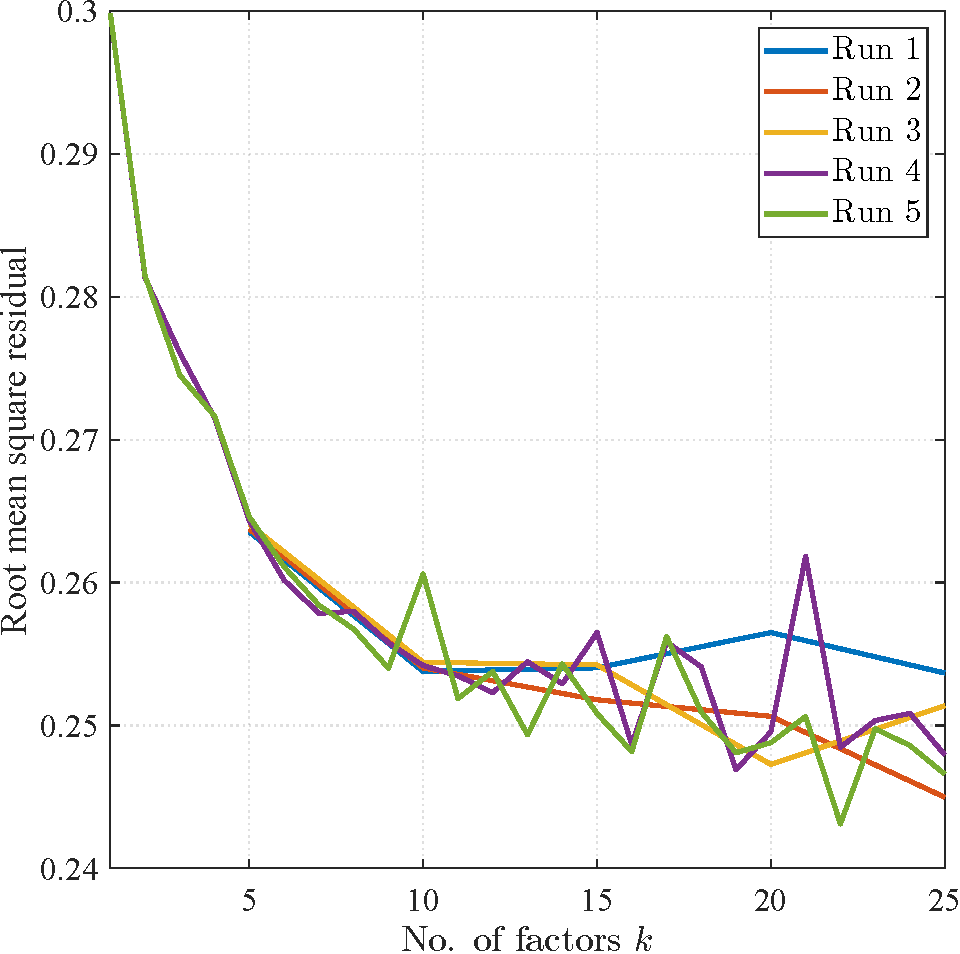
\includegraphics[width=0.99\columnwidth]{nnmf_elbow.pdf}
%		\hspace*{\fill}
%	\end{center}
%	\caption{\label{fig:nnmf_elbow} Elbow method to determine the number of factors for \ac{nnmf}.}
%\end{figure}
% ---

% Subsection ==================================================================
\subsection{Data collection}
% ---
\begin{figure*}[t!]
    \centering
    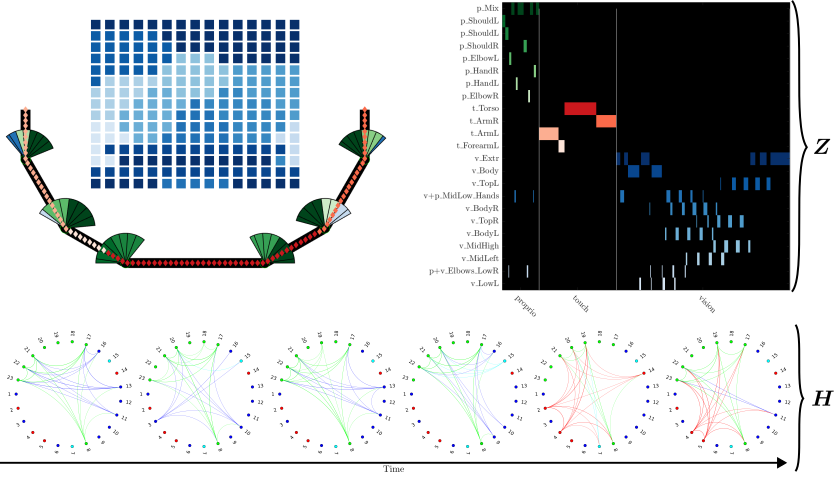
\includegraphics[width=0.95\textwidth]{fig/irm_results_figure.png}
    \caption{\textbf{Extracted sensorimotor modules and their \ac{dfc}.} \textsc{Right}: A total of $N_\text{c}=23$ clusters---representing functional modules---were found by the \ac{irm}, each assigned to a different color. We see a great separation of modules by modalities, e.g., proprioceptive, tactile, and visual modules. Sometimes, a specific part of the visual field can only be stimulated with specific hand or elbow angles. Hence, some visual modules can include proprioceptive sensors. \textsc{Left}: The \ac{irm} separates the visual field in functionally different portions, towards the middle of the torso for self-touch, left and right areas for waving the arms, a central area for touchings hands, and a top external area which is not reachable. \textsc{Bottom}: The matrix $\bm{H}$ from the \ac{irm} captures the \ac{dfc} between the $N_\text{c}$ modules.}
    \label{fig:irm_modules}
\end{figure*}

The agent described in Sec.~\ref{sec:the_embodied_agent} was simulated in MATLAB for a total time of 30 seconds with a sampling time of 1 ms (which corresponds to $N = 30,000$ data samples). Our experiment used a simple motor babbling strategy to stimulate the perceptual system and detect sensorimotor relationships via \ac{mi}. Each joint antagonistic pair received a periodic muscle activation command
% --- 
\begin{equation}\label{eq:motor_babbling_torques}
	\sigma(t) =  \text{tanh} \left( A_1 \text{sin}\left(\omega_0 t\right) + A_2 \text{sin}\left(2\omega_0 t\right) + A_3 \text{sin}\left(4\omega_0 t\right) \right);
\end{equation}	
% ---
with $A_i \sim \mathcal{U}(-1,1)$, the base frequency $\omega_0 = 2\pi/T_0$, and $T_0=2$ seconds.

% Subsection ==================================================================
%------
% \begin{figure*}[h!]
%     \centering
%     \begin{minipage}{0.32\textwidth}
%         \centering
%         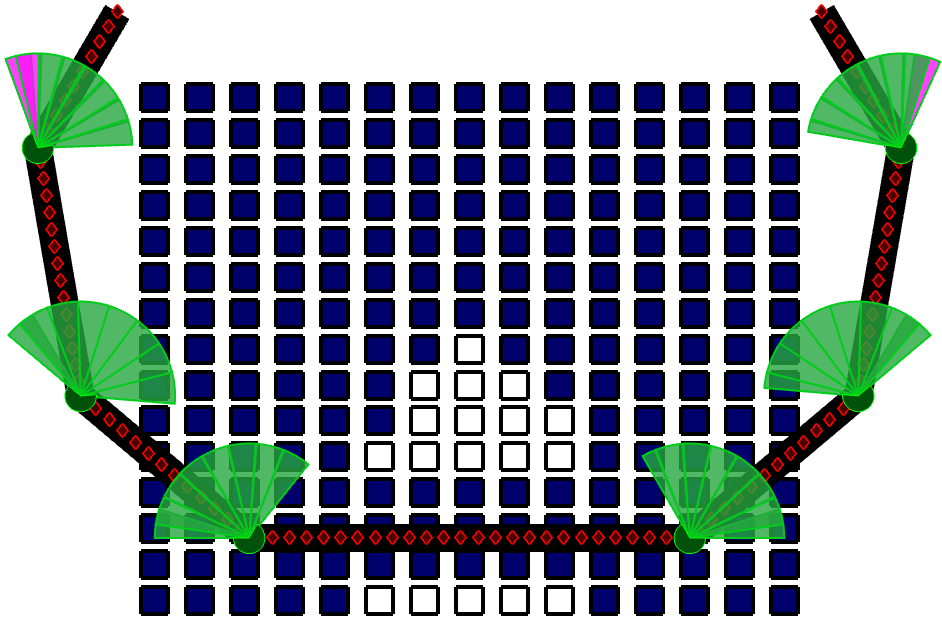
\includegraphics[width=\linewidth]{fig/modules_repr_v.png}
%         \textbf{(A) Visual module (vbody)}
%     \end{minipage}
%     \hfill
%     \begin{minipage}{0.32\textwidth}
%         \centering
%         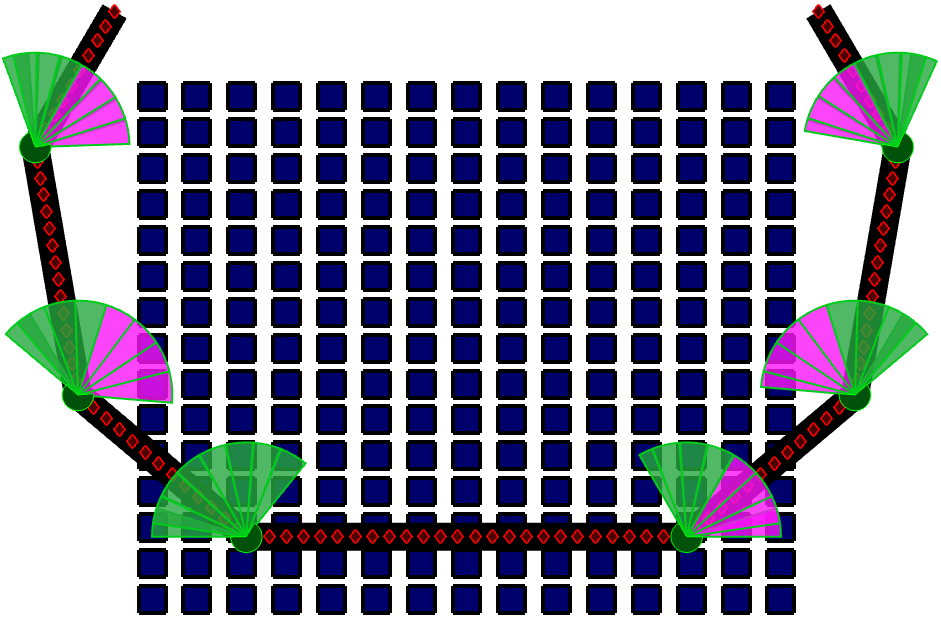
\includegraphics[width=\linewidth]{modules_repr_p.png}
%         \textbf{(B) Proprioceptive module}
%     \end{minipage}
%     \hfill
%     \begin{minipage}{0.32\textwidth}
%         \centering
%         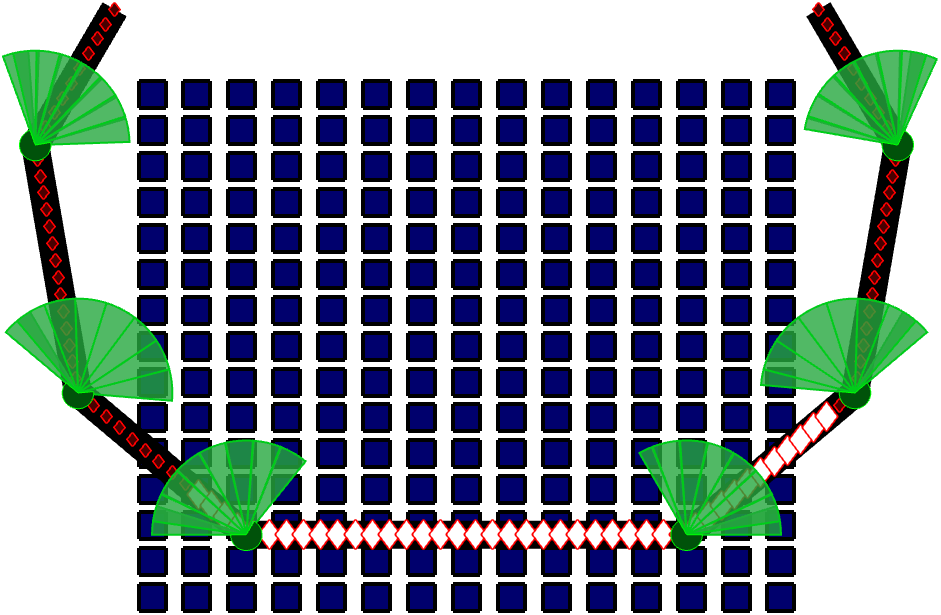
\includegraphics[width=\linewidth]{modules_repr_t.png}
%         \textbf{(C) Tactile module}
%     \end{minipage}
    
% %     \caption{Example of sensory clusters or modules obtained from the IRM. In white or pink are the sensors groups}
% %     \label{fig:three_images}
% \end{figure*}
\subsection{Sensorimotor modules and \ac{dfc}}
To compute the \ac{imi}, we used sensor signals sampled at 100 Hz and a sliding window of $T = 0.1$ seconds, i.e., the previously seen 10 samples. This short memory was stored in a buffer. The selection of a relatively short time window is motivated by tactile events often occurring within a short timescale. In this work, we used a binning strategy to compute the matrix $\bm{\mathcal{I}}$ at each time. For the actual computation of the \ac{mi}, we used the open-source MATLAB package \emph{Mutual information computation} \cite{PengMutualInformationcomputation}. Consequently, to compute $\bm{Z}$ and $\bm{H}$, we use the MATLAB-written package for Bayesian community detection available in \cite{Morup2025IRM}. 

Fig.~\ref{fig:irm_modules} depicts the output $\bm{Z}$ of the \ac{irm}. It found $N_\text{c} = 23$ functional modules corresponding to clusters of sensory signals with high information sharing (i.e., high \ac{imi}). We generally observe a clear separation of the sensory modalities into proprioception, touch, and vision. A few modules clustered visual and proprioceptive information together. Such modules originate from situations when the visual location of the hands is solely related to proprioceptive sensory inputs. It is worth noting the uneven number of elements across the modules. For example, the number of elements in the proprioceptive clusters in Fig.~\ref{fig:irm_modules} is smaller than in visual or tactile modules. This indicates that the signals in the proprioceptive modules carry a higher information-sharing level than modules that group a larger number of signals from other sensory modalities.
% ---
% \begin{figure*}[t!]
% 	\begin{center}
% 		\hspace*{\fill}
% 		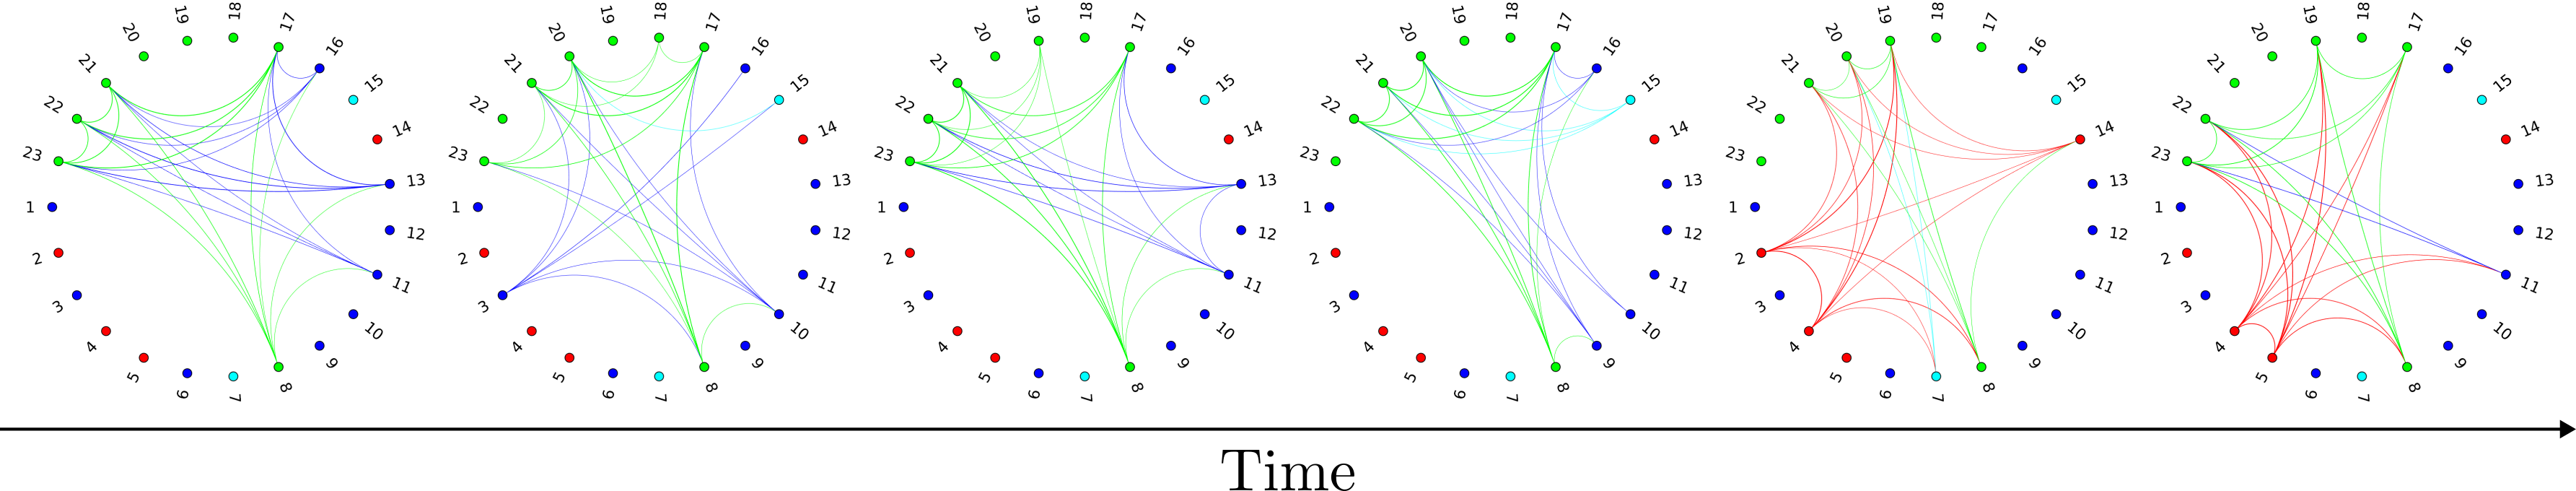
\includegraphics[width=0.9\textwidth]{fig/example_dfc.png}
% 		\hspace*{\fill}
% 	\end{center}
% 	\caption{\textbf{\Acl{dfc} from the \ac{irm}.} Exercpt from the time evolutoin of the connectivity between the modules found by the \acl{irm}.}
% \end{figure*}
% ---

% Subsection ==================================================================
\subsection{Fundamental motor behaviors and \ac{nnmf}}
% ---
\begin{figure*}[!t]
	\begin{center}
		\hspace*{\fill}
		% 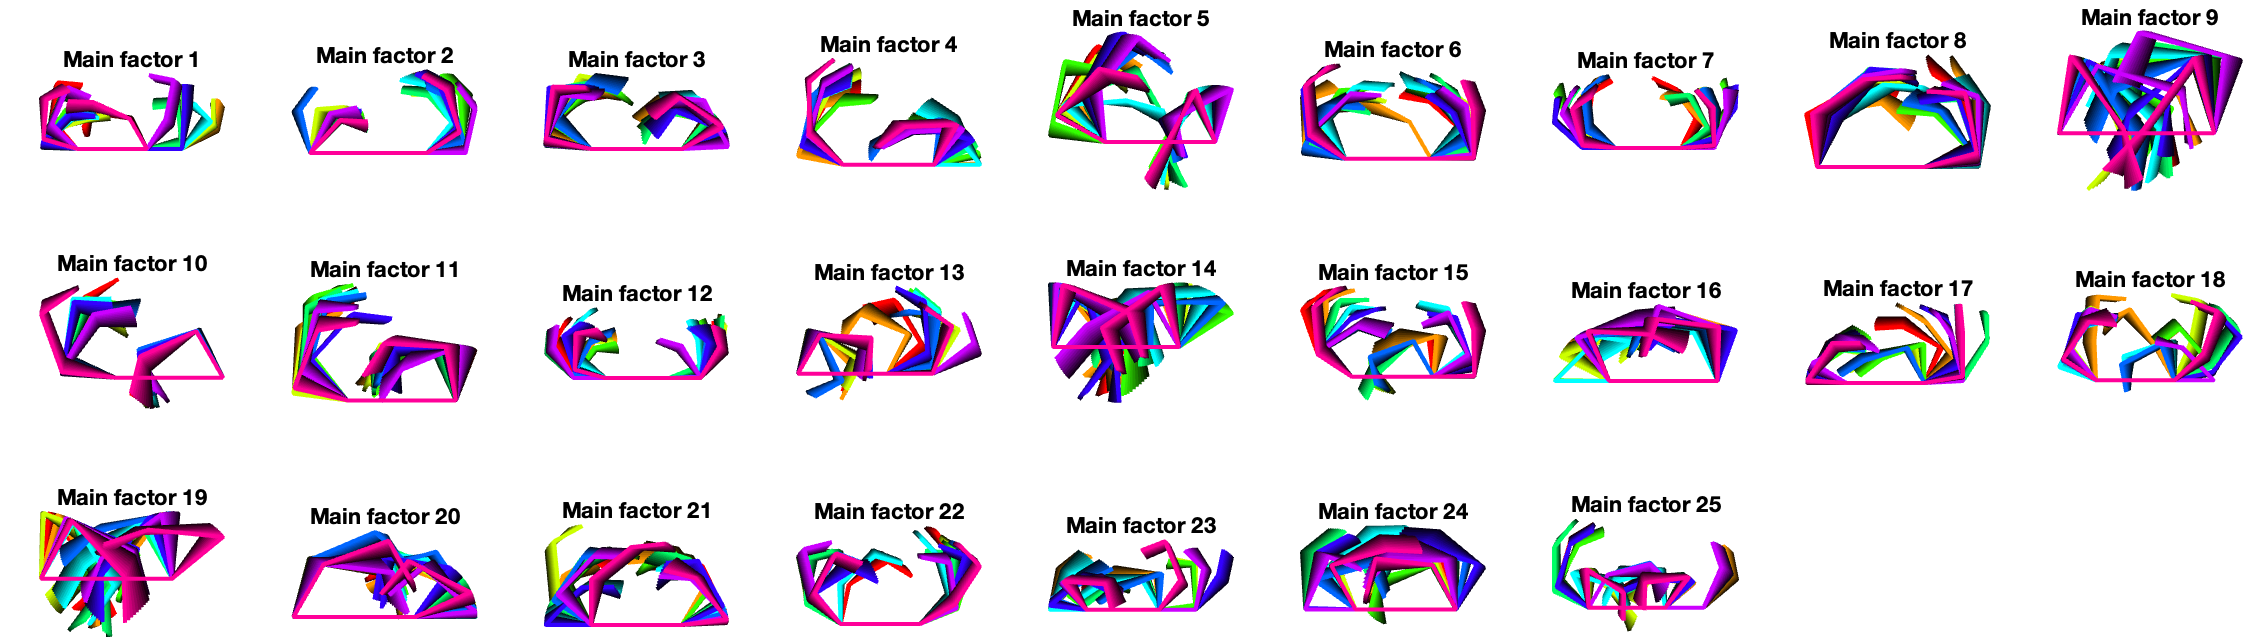
\includegraphics[width=0.95\textwidth]{fig/movement_mainfactors_horizontal.png}
        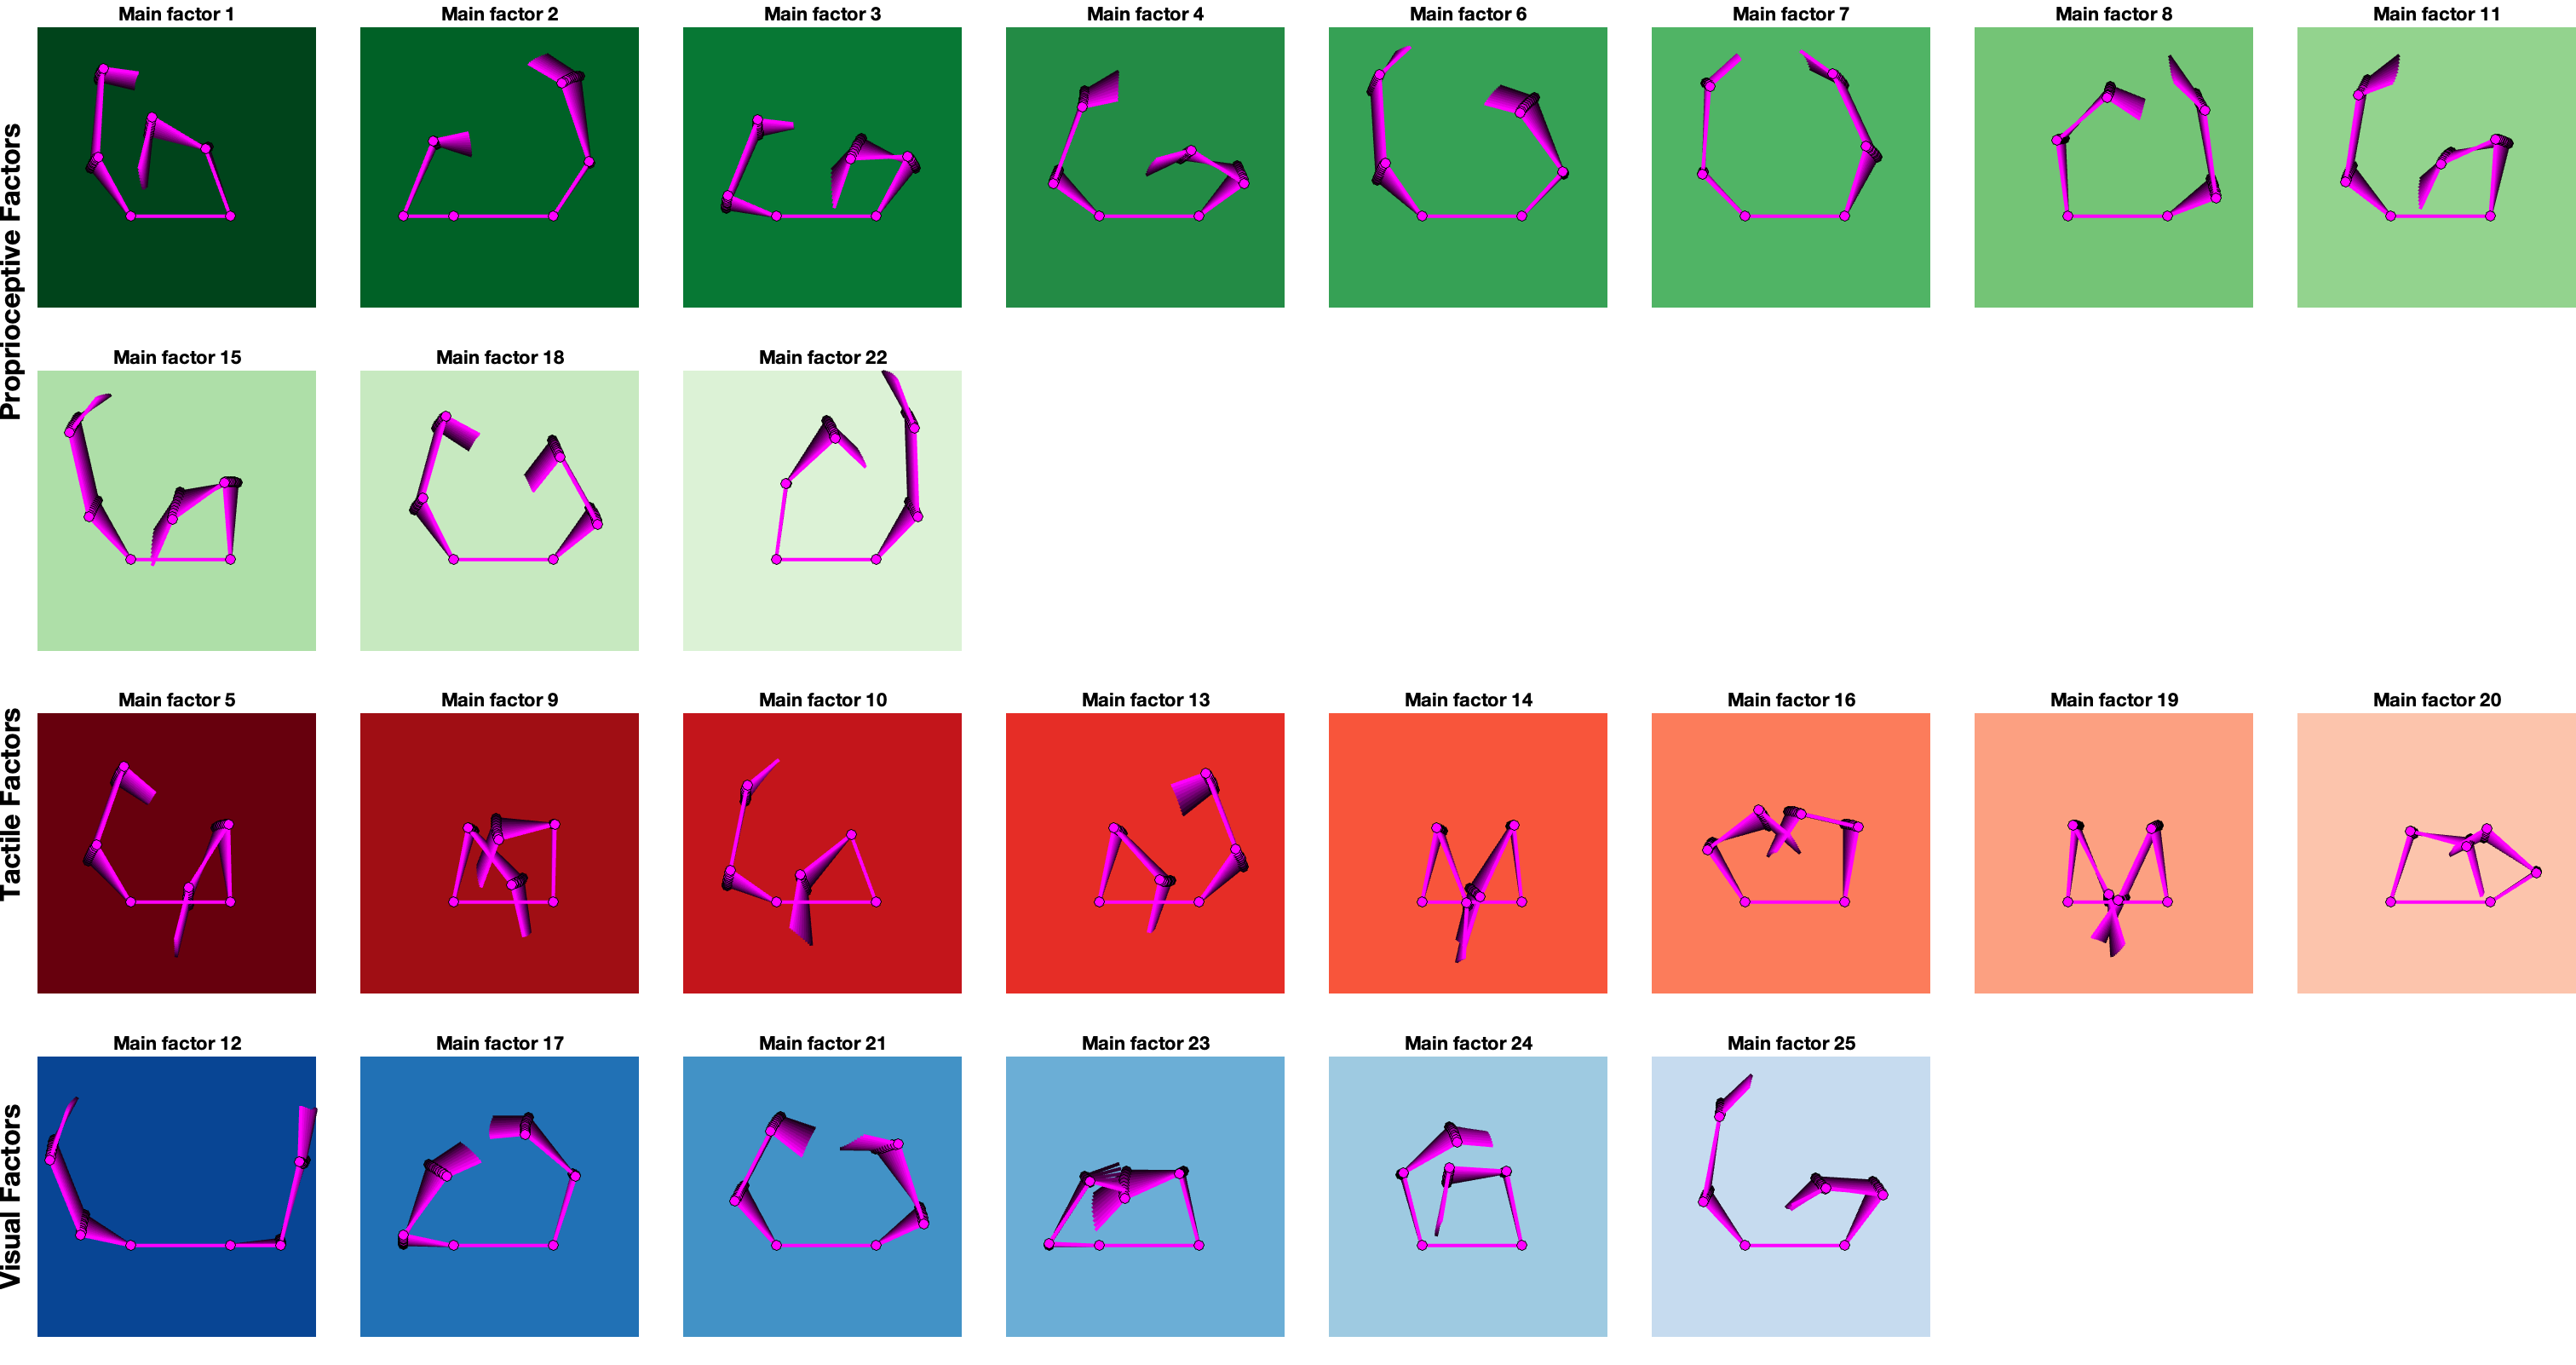
\includegraphics[width=1\textwidth]{fig/mainfactors_represente.png}
		\hspace*{\fill}
	\end{center}
	\caption{\textbf{The factors and associated behaviors.} Different events during exploration link to a given factor; for example, pure proprioception (no touch), contact with left arm, right arm, and both arms.}
    \label{fig:main_factors}
\end{figure*}
% ---
% One crucial question is the number of factors $k$ used to approximate the $\bar{\bm{H}}$. We chose $k$ following the elbow method as in \cite{Phalen2020Nonnegativematrix} by performing \ac{nnmf} for ascending values of $k$ and selecting the value where the residual error is not reduced any further.
From the link densities matrix $\bar{\bm{H}}$ between all modules, we apply \ac{nnmf}. One crucial question is the number of factors $k$ used to approximate the $\bar{\bm{H}}$. We chose $k$ following the elbow method as in \cite{Phalen2020Nonnegativematrix} and obtain a set of $N_\text{f} = 25$ nonnegative factors\\ $\bm{F} = [ \bm{f}_1 \cdots \bm{f}_i \cdots \bm{f}_{N_\text{f}}]$ and their corresponding scores $\left\lbrace w_i(k)\right\rbrace^{N_\text{f}}_{i=1}$
that decompose the link densities:
% ---
\begin{equation}
    \bar{\bm{h}}(k)\approx \sum_{i=1}^{N_\text{f}} w_i(k)\cdot\bm{f}_i.
\end{equation}
% ---
\myhl{HAve a talk here about how the factors are computed. choice of nb of factors, are they orthogonal etc..}
The factors in $\mathbf{F}$ are ordered by their contribution to the reconstruction of the link densities matrix in Eq.~\ref{eq:nnmf}, which is computed for each factor $i$, as the total score energy
% ---
\begin{equation}
    E_i =  \sum_{k=1}^N w_i(k)^2.
x\end{equation}
% ---
For each window of 10 samples where the \ac{imi} between all sensors is computed, we get one score for each factor $\bm{f}_i$. The sum of all factors weighted by their score approximates the current link density. The main factor corresponds to that with the highest score, e.g., the highest contribution in the link density. In the illustrative Fig.~\ref{fig:main_factors}, we show some example motor behaviors that led each of the factors to be the main factor.

%---
\subsection{Transition between main factors}
% ---
\begin{figure*}
    \centering
    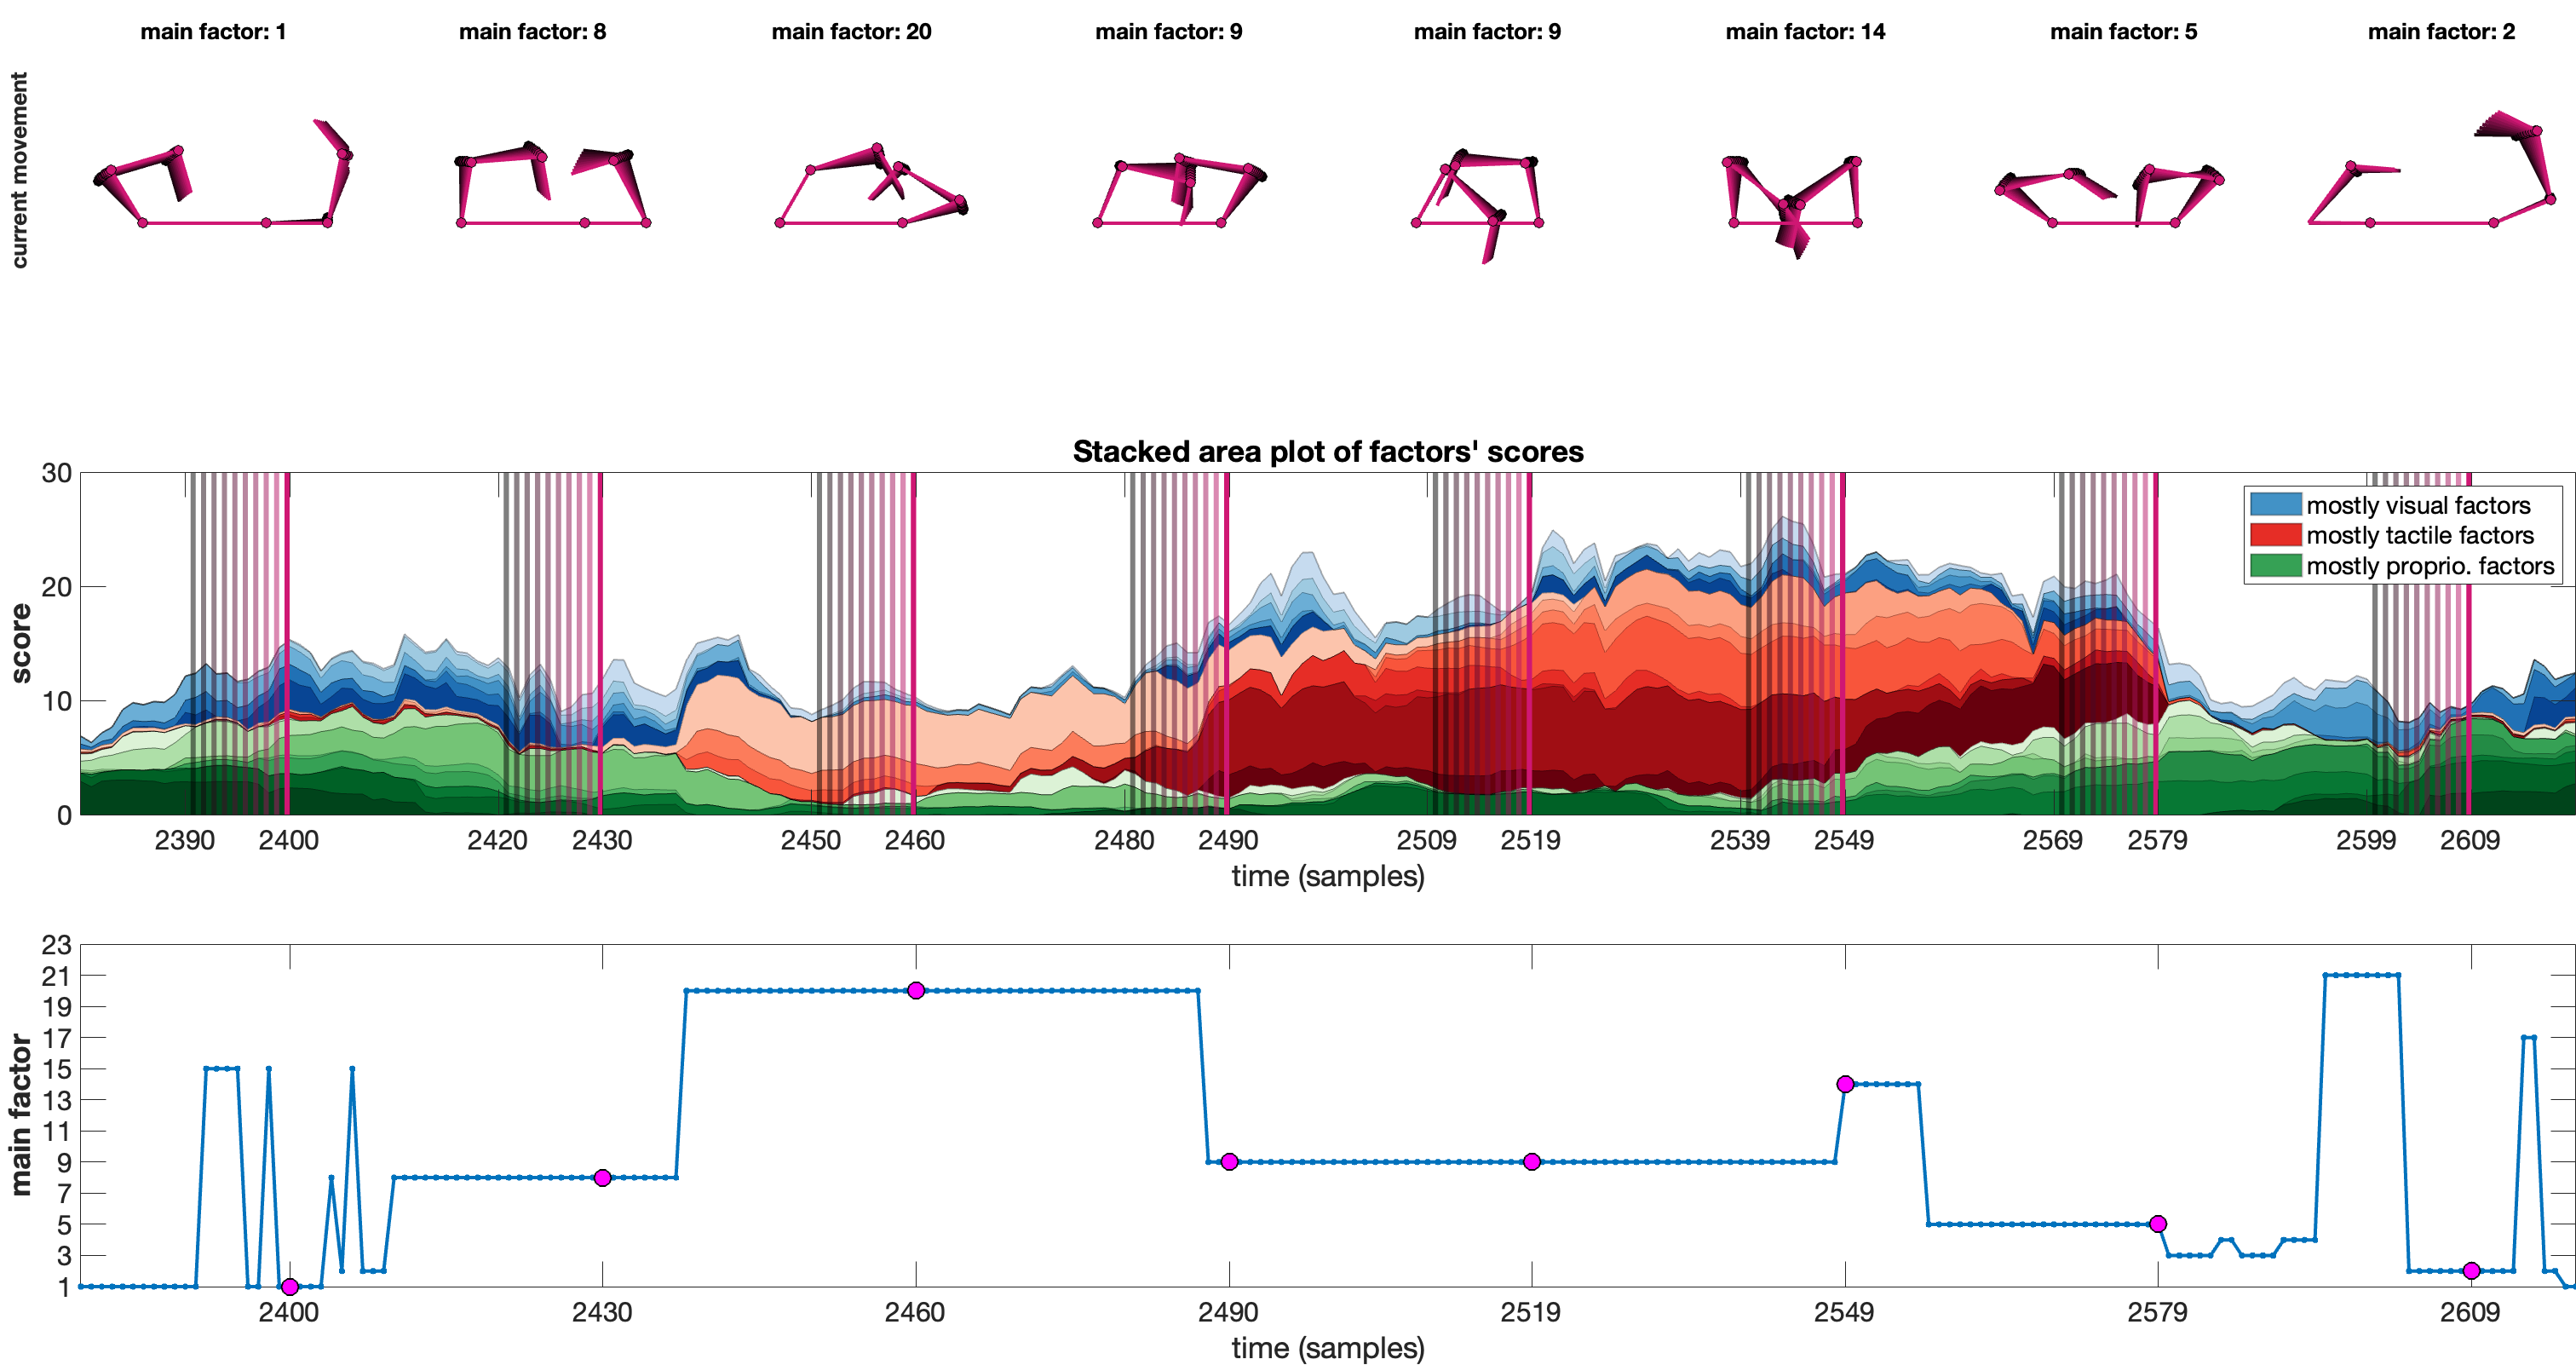
\includegraphics[width=.99\textwidth]{fig/factors_example_time.png}
    \caption{Example of possible interpration of the main factors. \textsc{Top}: agent's behavior at 8 different moments, the movement is 10 samples long, it corresponds to the time window on which the IMI is computed, and shown in shades of pink from darker/older to lighter/newer. The agent goes from waving the arms to hands touching, two hands touching the torso, right hand touching the torso and finally back to no-touch. \textsc{Middle}: stacked plot of each factors scores. In shades of blue are represented the factors with high sensitiviy to connection with visual modules, resp. red for tactile modules and green for proprioceptive. \textsc{Bottom}: evolution of the main factor, e.g. factor with the highest contribution to the estimation of the link density matrix $\bm{H}$. The main factor can be linked to the current behavior (top row).}
    \label{fig:factors_time}
\end{figure*}
% =============================================================================
%                                                                             |
%                                                                             |

% =============================================================================
%                                                                             |
%                                                                             |
% ------------------------------- SECTION ------------------------------------|
%                                                                             |
%                                                                             |
% =============================================================================
\section{On automatic behavior characterization}
\begin{itemize}
    \item How can we use the behaviors 
\end{itemize}
% ---

% =============================================================================
%                                                                             |
%                                                                             |
% ------------------------------- SECTION ------------------------------------|
%                                                                             |
%                                                                             |
% =============================================================================
\section{Conclusion}
This work introduced a framework for analyzing the \acl{dfc} among an embodied agent's multimodal sensory signals to uncover underlying structures in its sensorimotor interactions. By leveraging \acl{imi}, we captured the time-varying functional connections between proprioceptive, tactile, and visual signals, revealing fundamental sensorimotor relationships. By applying an \acl{irm}, we identified 23 sensorimotor modules and their evolving connectivity, represented by the link density matrix $\bm{H}$. To further interpret these dynamic interactions, we employed \acl{nnmf}, which decomposed the connectivity patterns into 25 additive factors (subgraphs, $\bm{f}_i$) and their corresponding temporal coefficients ($w_i(k)$).

Each of the $N_\text{f}$ factors in $\bm{F}$ can be interpreted as a basis \ac{fc} graph, capturing distinct states of information sharing between the $N_\text{c}$ sensorimotor clusters. These factors also encode fundamental movement primitives, representing the agent’s interactions with its body and environment. More broadly, they serve as proxies for \acp{smc} that emerge during motor babbling. At any given time, the agent’s observed interaction patterns can be viewed as a weighted combination of these \acp{smc}, governed by the entries of the coefficient matrix $\bm{W}$. By extracting structured representations of an embodied agent’s sensorimotor dynamics, our approach demonstrates the effectiveness of combining information-theoretic measures (\acl{mi}), Bayesian nonparametric models (\acl{irm}), and high-dimensional analysis (\ac{nnmf}) in studying \acp{smc}. Ultimately, our findings provide new insights into the relationship between embodiment and behavior, contributing to the broader understanding of how agents acquire and structure sensorimotor knowledge.

Despite its contributions, this study has certain limitations. The framework relies on motor babbling as the motion policy for collecting sensorimotor signals. While effective for exploration, alternative strategies---such as goal-directed or active exploration---could improve the ability to capture and reproduce specific sensorimotor behaviors. Inspired by \cite{Kanazawa2023Openendedmovements}, one promising approach would be to record motion data from real infants, map it onto musculoskeletal models to extract proprioceptive and tactile signals, and then apply our framework to uncover underlying motor behaviors. Additionally, our framework currently operates offline, requiring pre-collected data for analysis. Developing an online implementation capable of dynamically adapting parameters---such as the number of clusters or factors---remains an open challenge. This adaptability becomes particularly important as the agent's motor policy evolves, potentially revealing new fundamental behaviors (i.e., factors from the \ac{nnmf}). Moreover, given the additive nature of these factors, newly discovered ones could gradually replace older ones, reflecting the agent’s ongoing adaptation to its environment. Addressing these limitations in future work could enhance the framework’s applicability, particularly for real-time learning and adaptive sensorimotor behavior discovery.

% Each of the $N_\text{f}$ factors in $\bm{F}$ can be interpreted as a basis \ac{fc} graph capturing a state of information sharing between the $N_\text{c}$ sensorimotor clusters. They also encode interaction patterns---fundamental movement primitives---of the agent with its body. These patterns can also be understood as proxies that represent \acp{smc} that emerge during the motor babbling phase. The actual observed interaction patterns of the agent at a given time instant can be thought of as an aggregation of the \acp{smc} using the entries of the coefficient matrix $\bm{W}$. Via the factors $\bm{F}$, our approach demonstrates its suitability to extract structured representations of an embodied agent’s sensorimotor dynamics. Ultimately, our findings highlight the potential of information-theoretic metrics (the \acl{mi}), Bayesian nonparametric models (the \acl{irm}) and high-dimensional analysis (\ac{nnmf}) in studying sensorimotor contingencies, offering new insights into the relationship between embodiment and behavior. Future work will focus on extending this framework for online implementation and exploring active exploration strategies to enhance sensorimotor learning.

\printbibliography 
\end{document}